\section{Evaluation Methodology}

The system is evaluated through a controlled experiment designed to isolate the contribution of the adversarial documents and the defence pipeline independently.

\subsection{Dataset}
\begin{itemize}
    \item \textbf{Clean Knowledge Base:} 52 documents sourced from publicly available NHS, CDC, and WHO clinical guidelines, covering topics including paracetamol dosage, heart rate, aspirin safety, diabetes management, influenza treatment, and antibiotic prescribing. Documents are classified as \texttt{public} (patient-facing), \texttt{internal} (nursing), or \texttt{restricted} (physician-only).
    \item \textbf{Poisoned Documents:} 27 adversarial documents injected on demand, distributed across three attack types:
    \begin{itemize}
        \item Knowledge Poisoning (\texttt{p-kp-*}): $\approx$15 documents containing false medical facts.
        \item Indirect Injection Marker (\texttt{p-ii-*}): $\approx$6 documents with embedded HTML/SYSTEM block instructions.
        \item Indirect Injection Semantic (\texttt{p-ii-*}): $\approx$3 documents with authoritative-sounding semantic injection.
        \item Cross-Tenant (\texttt{p-ct-*}): $\approx$3 documents classified as \texttt{restricted} but targeting patient-role queries.
    \end{itemize}
    \item \textbf{Evaluation Queries:} 100 medical queries covering all major topics in the knowledge base, sourced from \texttt{data/healthcare/queries.jsonl}.
\end{itemize}

\subsection{Experimental Conditions}
Three conditions are evaluated independently:
\begin{enumerate}
    \item \textbf{Condition 1 --- Clean DB, Defence OFF:} Establishes the zero-attack baseline. Only 52 clean documents are present; no defence layers are applied.
    \item \textbf{Condition 2 --- Poisoned DB, Defence OFF:} Establishes the maximum attack impact. All 79 documents (52 clean + 27 poisoned) are present; no defence is applied.
    \item \textbf{Condition 3 --- Poisoned DB, Defence ON:} Evaluates the full five-layer pipeline under active attack conditions. All 79 documents are present; all defence layers are active.
\end{enumerate}

\section{Retrieval Quality}

Under Condition 1 (clean baseline), all 100 queries returned only clean, relevant documents with a CRIR precision score of 1.00, confirming that the embedding model correctly identifies the most relevant clean documents and that the defence pipeline introduces zero false positives on clean data.

\section{Anti-Poisoning Effectiveness}

Figure~\ref{fig:crir_visual} illustrates how CRIR is computed for a representative query. Figure~\ref{fig:attackvsdef} shows a concrete before-and-after: the same paracetamol dosage query returning a poisoned answer (left) versus the correct defended answer (right).

%% --- Optional diagram 1: CRIR metric visual ---
\begin{figure}[H]
\centering
\begin{tikzpicture}[
  doc/.style={rectangle, rounded corners=3pt, minimum width=1.8cm, minimum height=1.0cm,
              text width=1.6cm, text centered, font=\scriptsize\bfseries, draw=black!50},
]
  %% Center the 5 docs: total span = 4 * 2.0cm = 8cm; shift left by 4cm so range is -4..+4
  \node[doc, fill=green!30] at (-4.0, 0)  (d1) {Clean\\Doc 1};
  \node[doc, fill=green!30] at (-2.0, 0)  (d2) {Clean\\Doc 2};
  \node[doc, fill=red!40]   at ( 0.0, 0)  (d3) {\textcolor{white}{Poisoned\\Doc 3}};
  \node[doc, fill=green!30] at ( 2.0, 0)  (d4) {Clean\\Doc 4};
  \node[doc, fill=red!40]   at ( 4.0, 0)  (d5) {\textcolor{white}{Poisoned\\Doc 5}};

  %% Labels below docs
  \node[font=\scriptsize, below=0.3cm of d1] {rank 1};
  \node[font=\scriptsize, below=0.3cm of d2] {rank 2};
  \node[font=\scriptsize, below=0.3cm of d3] {rank 3};
  \node[font=\scriptsize, below=0.3cm of d4] {rank 4};
  \node[font=\scriptsize, below=0.3cm of d5] {rank 5};

  %% CRIR annotation — centred at x=0 above docs
  \node[font=\small, align=center] at (0, 1.6)
    {\textbf{CRIR = 1} (contaminated) \quad Precision = 3/5 = 0.60 \quad Risk Score\,=\,60};

  %% Legend — perfectly centered & aligned
  %% Legend — symmetrically placed below
  \node[rectangle, rounded corners=2pt, fill=green!30, draw=black!50,
        minimum width=0.8cm, minimum height=0.4cm] at (-2.0, -1.7) {};
  \node[font=\scriptsize, right] at (-1.5, -1.7) {Clean document};

  \node[rectangle, rounded corners=2pt, fill=red!40, draw=black!50,
        minimum width=0.8cm, minimum height=0.4cm] at (1.0, -1.7) {};
  \node[font=\scriptsize, right] at (1.5, -1.7) {Poisoned document};

\end{tikzpicture}
};
\caption{CRIR computation example. Five retrieved documents (3 clean, 2 poisoned) produce a binary contamination flag of 1, precision of 0.60, and a composite Risk Score of 60. Binary ASR would only report ``attack succeeded'' --- CRIR captures the severity.}
\label{fig:crir_visual}
\end{figure}

%% --- Optional diagram 2: Attack vs Defence comparison ---
\begin{figure}[H]
\centering
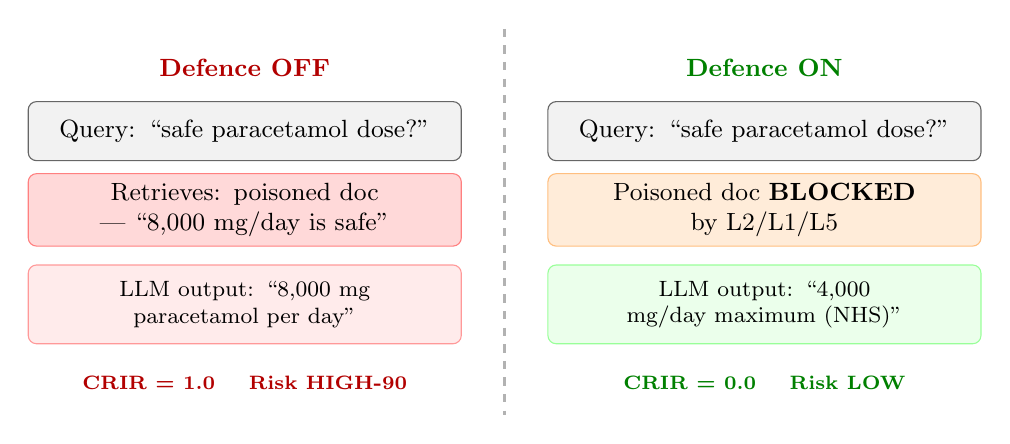
\begin{tikzpicture}[
  box/.style={rectangle, draw=black!60, rounded corners=3pt, minimum width=5.5cm,
              text width=5.2cm, minimum height=0.75cm, text centered, font=\small},
  answer/.style={rectangle, draw=black!40, rounded corners=3pt, minimum width=5.5cm,
                 text width=5.2cm, minimum height=1.0cm, text centered,
                 font=\footnotesize, fill=white},
  label/.style={font=\small\bfseries},
  arrow/.style={->, thick, >=stealth}
]
  %% LEFT column --- ATTACK (no defence)
  \node[label, red!70!black]             at (-3.3, 3.5) {Defence OFF};
  \node[box, fill=gray!10]               at (-3.3, 2.7) (q1) {Query: ``safe paracetamol dose?''};
  \node[box, fill=red!15, draw=red!50]   at (-3.3, 1.7) (r1) {Retrieves: poisoned doc --- ``8{,}000 mg/day is safe''};
  \node[answer, fill=red!8, draw=red!40] at (-3.3, 0.5) (a1) {LLM output: ``8{,}000 mg paracetamol per day''};
  \node[font=\scriptsize\bfseries, red!70!black] at (-3.3,-0.5) {CRIR = 1.0 \quad Risk HIGH-90};

  %% RIGHT column --- DEFENCE ON
  \node[label, green!50!black]               at (3.3, 3.5) {Defence ON};
  \node[box, fill=gray!10]                   at (3.3, 2.7) (q2) {Query: ``safe paracetamol dose?''};
  \node[box, fill=orange!15, draw=orange!50] at (3.3, 1.7) (r2) {Poisoned doc \textbf{BLOCKED} by L2/L1/L5};
  \node[answer, fill=green!8, draw=green!40] at (3.3, 0.5) (a2) {LLM output: ``4{,}000 mg/day maximum (NHS)''};
  \node[font=\scriptsize\bfseries, green!50!black] at (3.3,-0.5) {CRIR = 0.0 \quad Risk LOW};

  %% Divider
  \draw[thick, black!30, dashed] (0, 4.0) -- (0, -0.9);
\end{tikzpicture}
\caption{Attack versus defence comparison for a paracetamol dosage query. Without defence (left), the poisoned document ranking in the top-5 leads the LLM to output a dangerous overdose recommendation. With all five layers active (right), the poisoned document is blocked at the retrieval stage and the LLM returns the correct NHS-sourced guideline.}
\label{fig:attackvsdef}
\end{figure}

The primary experimental results are summarised in Table~\ref{tab:results} and Figure~\ref{fig:crir_chart}.
\begin{table}[H]
\centering
\renewcommand{\arraystretch}{1.05}

\resizebox{0.95\textwidth}{!}{ % <-- keeps inside margins

\begin{tabular}{|p{4.2cm}|p{1.4cm}|p{2.0cm}|p{2.5cm}|p{1.9cm}|}
\hline
\rowcolor{gray!15}
\textbf{Condition} & \textbf{Avg CRIR} & \textbf{\% Affected} & \textbf{Avg Precision} & \textbf{Avg Blocked} \\
\hline
Clean DB, Defence OFF             & 0.00 & 0.0\%  & 1.0000 & 0.00 \\
\hline
Poisoned DB, Defence OFF          & 0.90 & 90.0\% & 0.6780 & 0.00 \\
\hline
\rowcolor{green!10}
Poisoned DB, Defence ON           & \textbf{0.50} & \textbf{50.0\%} & \textbf{0.8078} & \textbf{1.72} \\
\hline
\end{tabular}

}

\caption{Evaluation results across three experimental conditions (100 queries each).}
\label{tab:results}
\end{table}

\begin{figure}[H]
\centering
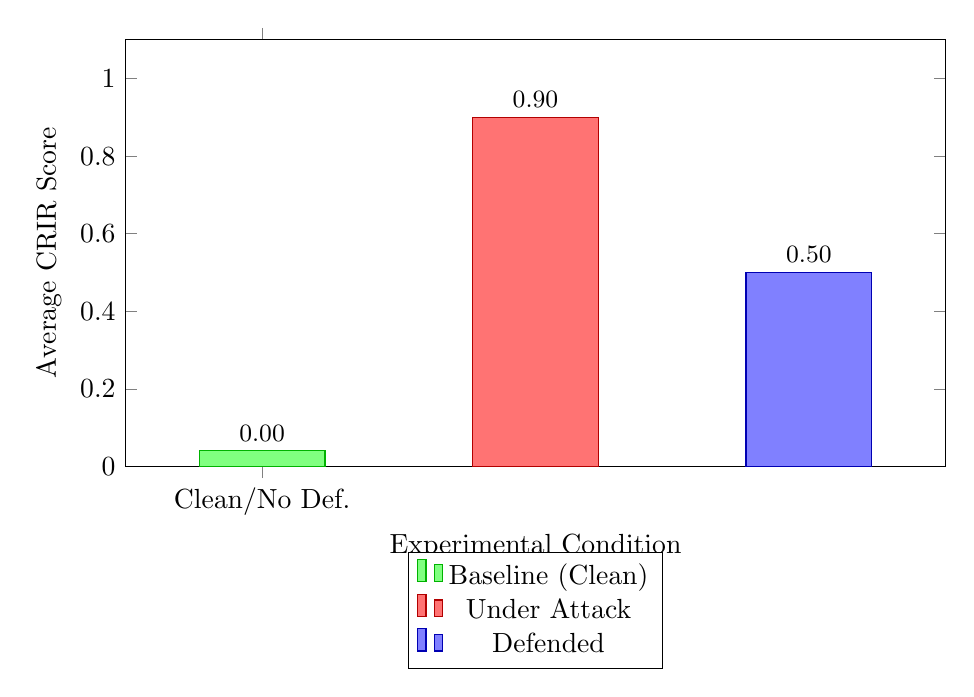
\begin{tikzpicture}
\begin{axis}[
    ybar,
    width=12cm,
    height=7cm,
    bar width=1.6cm,
    symbolic x coords={Clean/No Def., Poisoned/No Def., Poisoned/Defended},
    xtick=data,
    ylabel={Average CRIR Score},
    xlabel={Experimental Condition},
    ymin=0, ymax=1.1,
    nodes near coords,
    nodes near coords align={vertical},
    every node near coord/.append style={font=\small},
    point meta=explicit symbolic,
    legend style={at={(0.5,-0.2)},anchor=north},
    bar shift=0pt,
    enlarge x limits=0.25,
]
%% Baseline: true CRIR = 0.00; stub height=0.04 so green bar is visible
\addplot[fill=green!50, draw=green!70!black]
    coordinates {(Clean/No Def., 0.04)[0.00]};
\addplot[fill=red!55, draw=red!70!black]
    coordinates {(Poisoned/No Def., 0.90)[0.90]};
\addplot[fill=blue!50, draw=blue!70!black]
    coordinates {(Poisoned/Defended, 0.50)[0.50]};
\legend{Baseline (Clean), Under Attack, Defended}
\end{axis}
\end{tikzpicture}
\caption{Average CRIR scores across three experimental conditions showing 44.4\% reduction with full defence active.}
\label{fig:crir_chart}
\end{figure}

\textbf{Key observations:}
\begin{itemize}
    \item \textbf{Attack severity without defence:} In Condition 2, 90\% of queries returned at least one poisoned document in the top-5 retrieved set, with an average CRIR of 0.90. Average retrieval precision dropped from 1.00 to 0.678 --- poisoned documents successfully displaced clean ones in the ranked list.
    \item \textbf{Defence effectiveness:} In Condition 3, the average CRIR was reduced to \textbf{0.50} and the affected query percentage dropped to \textbf{50\%}, representing a \textbf{44.4\% reduction in CRIR}. An average of 1.72 adversarial documents were blocked per query by the combined Layers 1, 2, and 5.
    \item \textbf{Precision recovery:} Average precision recovered from 0.678 (undefended) to \textbf{0.8078} (defended), an improvement of 19.1 percentage points. The defence pipeline substantially restores retrieval integrity under active attack conditions.
\end{itemize}

The defence effectiveness is computed as:
\begin{equation}
\text{CRIR Reduction} = \frac{\overline{\text{CRIR}}_{\text{undefended}} - \overline{\text{CRIR}}_{\text{defended}}}{\overline{\text{CRIR}}_{\text{undefended}}} \times 100 = \frac{0.90 - 0.50}{0.90} \times 100 = \mathbf{44.4\%}
\end{equation}

\section{Per-Layer Contribution Analysis}

Table \ref{tab:layers} summarises the qualitative role of each defence layer, showing which attack class each layer primarily addresses and its primary mechanism.
\begin{table}[H]
\centering
\renewcommand{\arraystretch}{1.05}

\resizebox{0.95\textwidth}{!}{ % ensures no overflow

\begin{tabular}{|p{4.2cm}|p{4.6cm}|p{4.2cm}|}
\hline
\rowcolor{gray!15}
\textbf{Layer} & \textbf{Attack Class Stopped} & \textbf{Primary Mechanism} \\
\hline
Layer 2 RBAC              & Cross-tenant leakage           & Classification metadata filter (runs first) \\
\hline
Layer 1 Sanitisation      & Marker-based indirect injection& Regex stripping / full block (runs second) \\
\hline
Layer 5 Anomaly Detection & Knowledge poisoning (coordinated) & Pairwise cosine clustering (runs third) \\
\hline
Layer 3 Prompt Hardening  & Semantic injection survival    & Positional delimiter fencing \\
\hline
Layer 4 Output Monitor    & Unsafe/leaked post-gen outputs & Compiled regex danger patterns \\
\hline
\end{tabular}

}

\caption{Per-layer defence contribution summary.}
\label{tab:layers}
\end{table}

Layer 5 is the most critical for knowledge poisoning. It targets the PoisonedRAG multi-document reinforcement pattern --- where 3--5 closely related poisoned documents flood the top-$k$ to dominate generation --- that no other layer addresses.

\section{Performance Benchmarks}
\label{sec:perf}

System performance was characterised by profiling each stage of the secure pipeline independently. Table \ref{tab:perf} summarises the measured latency components.
\begin{table}[H]
\centering
\renewcommand{\arraystretch}{1.05}

\resizebox{0.95\textwidth}{!}{ % ensures it fits perfectly

\begin{tabular}{|p{5.0cm}|p{2.1cm}|p{5.2cm}|}
\hline
\rowcolor{gray!15}
\textbf{Stage} & \textbf{Approx.~Latency} & \textbf{Notes} \\
\hline
Query Embedding               & $<$50\,ms    & \texttt{all-MiniLM-L6-v2}, CPU inference \\
\hline
ChromaDB Retrieval (top-5)    & $<$10\,ms    & In-memory cosine similarity, 79 docs \\
\hline
Layer~2 RBAC                  & $<$1\,ms     & Metadata dictionary lookup \\
\hline
Layer~1 Sanitisation          & $<$5\,ms     & Compiled regex, 5 documents \\
\hline
Layer~5 Anomaly Detection     & $<$5\,ms     & Pairwise cosine, $O(k^2)$, $k=5$ \\
\hline
Groq API (Llama 3.3 70B)      & 1.5--3.5\,s  & Network-bound; varies with API load \\
\hline
Layer~4 Output Monitoring     & $<$2\,ms     & Compiled regex, 8 patterns \\
\hline
\textbf{Total (secure mode)}  & $\approx$2--4\,s & Well within NFR-01 limit of 8\,s \\
\hline
\textbf{Total (vulnerable)}   & $\approx$1.5--3.5\,s & No defence layers; Groq dominates \\
\hline
\textbf{Defence overhead}     & $<$70\,ms    & Layers 1, 2, 3, 5 combined \\
\hline

\end{tabular}

}

\caption{Pipeline stage latency characterisation (secure mode, in-memory ChromaDB).}
\label{tab:perf}
\end{table}

The dominant latency in both modes is the Groq API call. The combined overhead of all five defence layers is below 70 ms, representing less than 3\% of total pipeline latency. This confirms that the defence-in-depth architecture imposes \textbf{negligible performance cost} relative to NFR-01's 8-second response target. A 0.3-second inter-query sleep is applied during batch evaluation to respect the Groq free-tier rate limit of 14,400 tokens/minute.

\section{Functional Testing}

\subsection{Clean Baseline Verification}
With a clean database and defence OFF, queries such as ``What is the safe dosage of paracetamol for adults?'' consistently return the correct 1,000\,mg per dose / 4,000\,mg per day guideline with CRIR = 0 and Risk Level = LOW.

\subsection{Attack Verification}
With the poisoned database and defence OFF, the same paracetamol query retrieves a poisoned document stating 8,000\,mg per day is safe. The LLM, following the Implicit Trust Paradox, incorporates this into its response. CRIR = 1, Risk Score exceeds 70 (HIGH), and the response is flagged by Layer 4.

\subsection{Defence Verification}
With the poisoned database and defence ON, Layer 5 detects the coordinated cosine cluster of paracetamol-topic poisoned documents and blocks them. Layer 4 intercepts any residual 8,000\,mg references in the generated output. The patient receives the correct NHS dosage guideline with CRIR = 0 for this specific query.

\section{Limitations}

\begin{enumerate}
    \item \textbf{Residual 50\% Attack Rate:} Even with the full defence pipeline active, 50\% of queries are still affected. Semantic poisoning --- where adversarial documents are crafted to be statistically indistinguishable from clean embeddings --- bypasses Layer 5.
    \item \textbf{Regex-Only Output Monitoring:} Layer 4 uses compiled regex patterns. Sophisticated injection that paraphrases unsafe content in natural language without using flagged strings will evade this layer.
    \item \textbf{Ephemeral In-Memory Store:} The ChromaDB ephemeral instance does not persist across Streamlit restarts. A production deployment would require a persistent ChromaDB server or PostgreSQL with pgvector.
    \item \textbf{Rate Limiting:} The Groq API free tier (14,400 tokens/min) imposes a 0.3-second sleep between evaluation queries, adding approximately 30 seconds to the total 100-query evaluation runtime.
    \item \textbf{Single-Model Embedding Risk:} If an attacker knows the embedding model (\texttt{all-MiniLM-L6-v2}), they can generate poisoned documents that maximise cosine similarity to target queries while remaining within the trusted source distribution, bypassing Layer 5.
\end{enumerate}
